\chapter{Business-Cycle Indicators}
\label{chp:bcin}
\hypertarget{indicators}{}

\textbf{Tools:} Basic statistics (standard deviation, correlation); cross-correlation function.

\textbf{Key Words:} \textbf{Key Words:} Volatility; procyclical and countercyclical;  leading, lagging, and coincident. 

\textbf{Big Ideas:}
\vspace{-0.1in}
\begin{itemize}
\item Business cycle indicators are characterized by several properties:  procyclical and countercyclical,
leading and lagging.
\item Cross-correlation functions identify these properties.
\end{itemize}
\rule{\textwidth}{1pt}

Probably the leading use of macroeconomic data (and macroeconomists)
is forecasting:  predicting future movements in economic variables
so that businesses can decide how much to produce,
investors can decide how to allocate their assets,
and households can decide how much to spend.
The good news is that forecasting is possible;
we're not simply throwing darts at a board.
The bad news is that it's not easy;
even the best forecasters are far from perfect.

This chapter is devoted to short-term business-cycle
indicators --- variables that indicate changes in near-term economic conditions --- and how to use them.
In principle, we could be interested in many features of
the economy:  output, inflation, interest rates,
exchange rates, and so on.
We'll focus on output, but the methods can easily be applied
to other variables.
We look at the US, but similar ideas and methods apply to
any country with reliable data.


\section{Terminology}

We refer to the properties of economic indicators with two related sets of terms.
One set of terms
describes whether an indicator's movements
tend to come before or after movements in output.
We say an indicator {\it leads\/} output if
its ups and downs typically precede those of output,
and {\it lags\/} output if they come after.
An indicator whose movements are contemporaneous with those of output
is referred to as {\it coincident\/}.
Thus, the adjectives leading, lagging, and  coincident
describe the timing of an indicator's movements relative to those of output.
Looking ahead, you might guess that leading indicators are
most useful in forecasting.
The stock market, for example, is a common leading indicator;
it leads output by six to eight months, as we'll see shortly.


A second set of terms refers to
whether an indicator's movements
are positively or negatively correlated with output.
If the correlation is positive, we say it is {\it proccyclical\/};
if the correlation is negative, we say it is {\it countercyclical\/}.
%If its movements are unrelated to those in output,
%we say it is {\it acylical\/}.
Most indicators are procyclical:  employment, stock prices, \
housing starts, and so on.
The most common countercyclical indicators have to do with unemployment: Both the unemployment rate and new claims for unemployment insurance
 rise during recessions.

\section{Forecasting}

The classic forecasting problem goes something like this:
What do we expect the value of [some
economic variable] to be $k$ periods in the future?
Here, $k$ is any period of time you like, but
we're usually interested in anything from next week to a few years in
the future.

\begin{figure}
    \caption{US GDP and industrial production.}
    \label{fig:ip_gdp}%
    \centering
    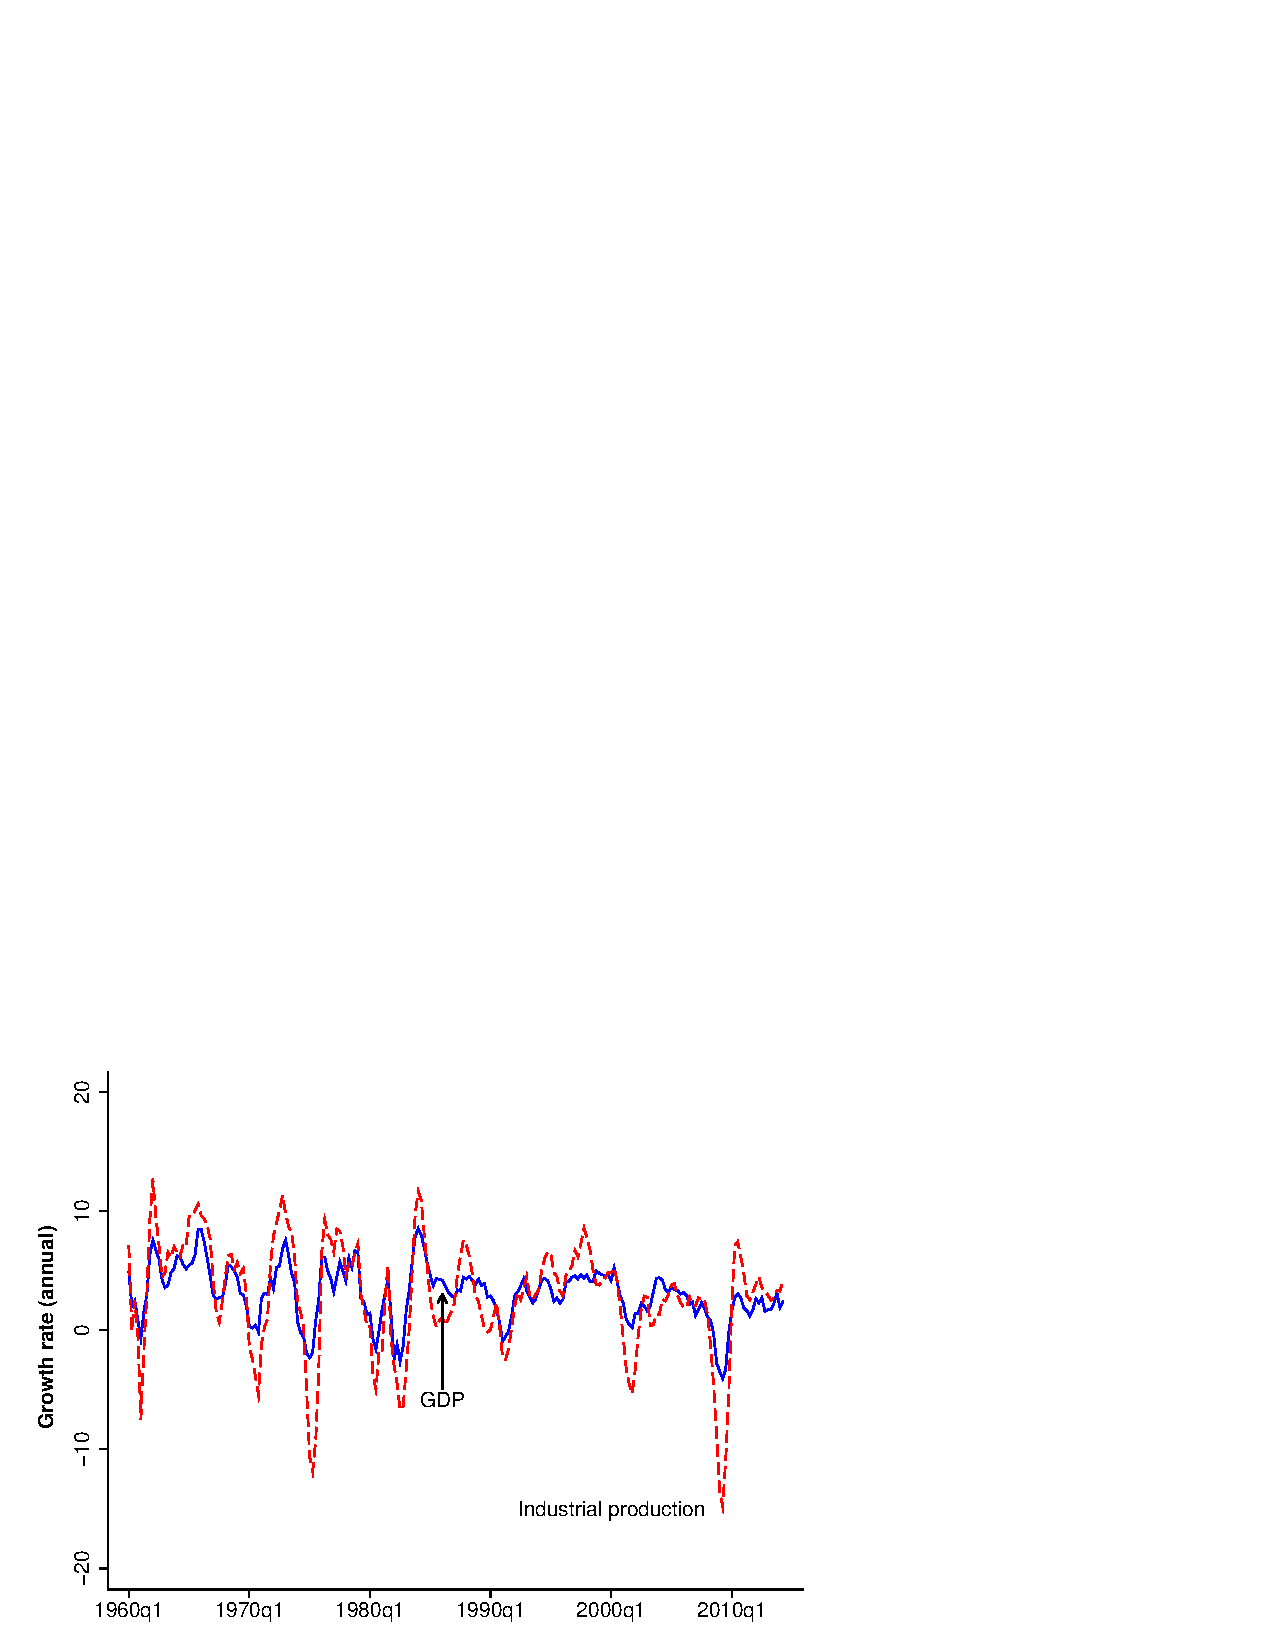
\includegraphics[width=0.8\textwidth]{Figures/us_gdp_indprod.pdf}
\end{figure}


If we're forecasting GDP, there's an extra difficulty because we don't
know the present or the recent past, much less the future. We've
seen, for example, that fourth-quarter GDP is first reported near
the end of the following January, and even that number is a
preliminary estimate. From the perspective of mid-January, then,
we need to ``forecast'' the previous quarter.


We're going to shortcut this difficulty (somewhat) by using the
monthly \href{http://research.stlouisfed.org/fred2/series/INDPRO?cid=3}{Industrial Production (IP)} index as a substitute for real
GDP, but the issue is a general one, in that the time lag in getting data
is both an issue in its own right and a  constraint on forecasting
the future. IP measures output in manufacturing, mining, and
utilities. More important, its fluctuations are strongly
correlated with those in GDP.  You can see that in
Figure~\ref{fig:ip_gdp}, which compares year-on-year growth rates
in GDP and IP (aggregated to a quarterly frequency). You will
notice that IP is more volatile than GDP but otherwise follows its
ups and downs reasonably well.  You may also notice some
differences between them in the recent past, which have been
traced to the rising importance of services in the US economy.  In
the US, IP is reported by the Federal Reserve in the middle of the
following month.  Data for December, for example, are available in
mid-January.  Using IP, therefore, gives us a shorter information
lag than GDP.  In addition, the monthly frequency gives us a finer
time interval for near-term forecasting.  For both reasons, we
will focus our discussion of forecasting on IP rather than, GDP,
although the same principles apply to both, as well as to other
macroeconomic and financial variables.

\section{Good indicators}

Good forecasts require good inputs.
One way to forecast a variable is with its own past.
Future growth rates of IP, for example, might be related
to current and past growth rates.
We can usually do better than that by adding other indicators
to our analysis.
Speaking generally,
a good indicator should have one or more of these properties:
%
\begin{itemize}

\item \textbf{Correlation.}  A good indicator is correlated with the
variable we are forecasting.

\item \textbf{Lead.} A good indicator leads the variable we are
forecasting.

\item \textbf{Timeliness.}  A good indicator is available quickly.

\item\textbf{Stability.}  A good indicator does not undergo major
revisions subsequent to its initial release, and its
relationship with the variable we are forecasting doesn't
change over time.

\end{itemize}
On the whole, measures of economic activity
(employment, for example)
tend to be strong on correlation and weak on timeliness (see the
discussion of GDP above) and stability (many economic series are
revised frequently).  The best ones lead the business cycle.  In
contrast, financial indicators (equity prices, interest rates) are
weaker on correlation but stronger on the other three properties:
They're typically available immediately, often lead the cycle, and
are not revised.
Various indexes of leading indicators combine multiple series with the
hope of getting the best from each.  The Conference Board's
quasi-official index of leading indicators is the most common example.



\section{Identifying good indicators}

How do we identify indicators with high potential?
We'll use another bit of terminology that leads to an extremely useful
graphical representation of the dynamic relation between two variables:
the {\it cross-correlation function\/} (ccf).

You may recall that the correlation between two variables
($x$ and $y$, say) is a measure of
how closely they are related in a statistical sense.
If the correlation is (say) 0.8,
then observations with large values of $x$
tend also to have large values of $y$.
If the correlation is 0.4, this association is weaker.
And if the correlation is --0.8,
observations with large values of $x$
tend to have small values of $y$ --- and vice versa.

\begin{figure}[h!]
    \caption{Cross-correlations: the S\&P 500 and industrial production.}
    \label{fig:ccf-sp500}%
    \centering
    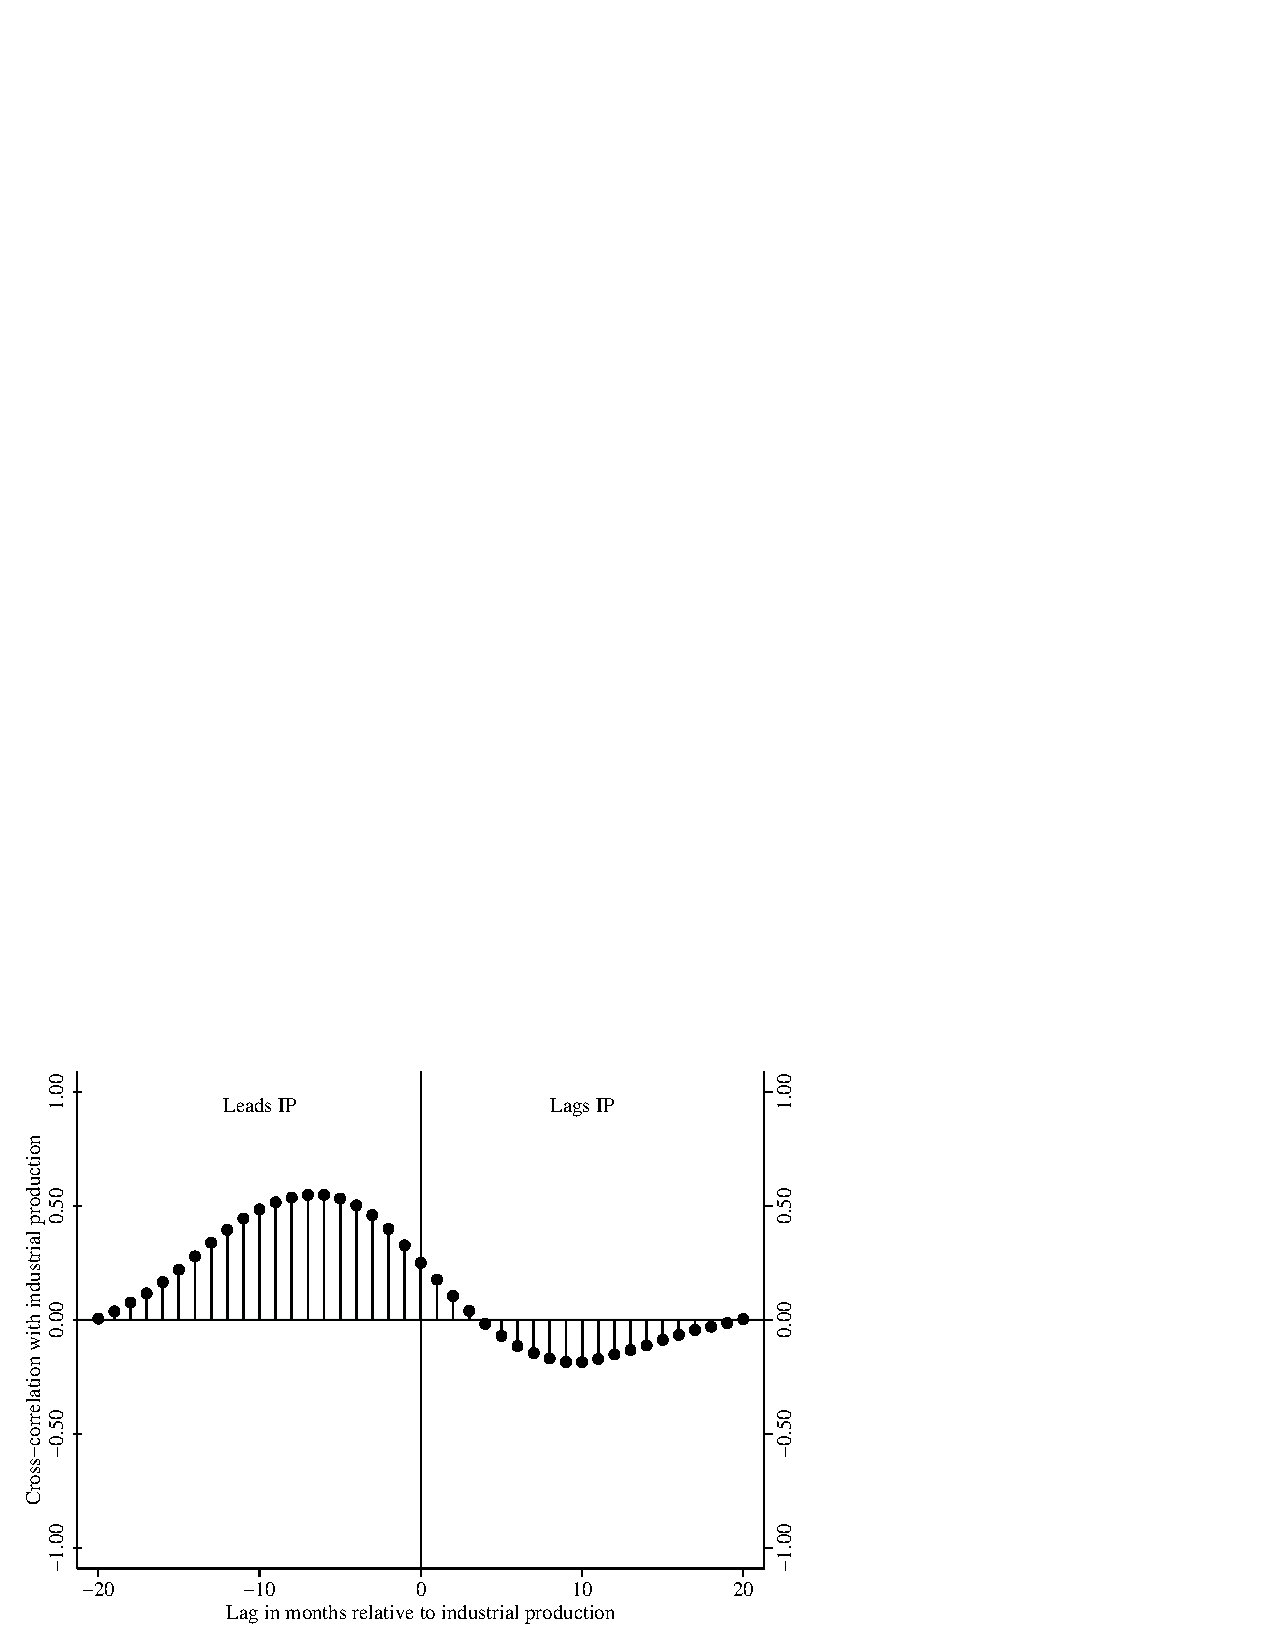
\includegraphics[width=0.8\textwidth]{Figures/xcsp500.pdf}

    \begin{minipage}{0.8\textwidth}
    \footnotesize{Both series are year-on-year growth rates for the period
    1960-present.
    The large correlations to the left tell us that
    the S\&P 500 index is a good indicator of future industrial production.}
    \end{minipage}
\end{figure}

The cross-correlation function extends the concept of correlation
to the timing of two indicators.
Specifically, consider the correlation between $x$ at date $t$
and $y$ at date $t-k$.  If $k$ is negative,
then we're talking about the correlation
between $x$ now and $y$ $k$ periods in the future.
If $k$ is positive, we have the correlation between $x$ now and
$y$ $k$ periods in the past.
By looking at the pattern of correlations,
we can identify indicators $x$ that tend to lead the variable $y$.
We refer to $k$ as the lag of $y$ vs $x$,
but if $k$ is negative it refers to a lead.
Mathematically, we write
\[
    \mbox{ccf}(k) \;=\;  \mbox{\it corr\/} (x_t,y_{t-k}) .
\]
Typically, we would graph this against $k$, with $k$ starting
with a negative number and moving to positive numbers.
The pattern of correlations tells us whether an indicator $x$
leads or lags (on average) a variable $y$.


Let's move from the abstract to the concrete to make sure we
understand what the ccf represents.
[You might want to work your way through this paragraph slowly,
as it's important.]
We calculate the year-on-year growth rates of the \href{http://research.stlouisfed.org/fred2/series/SP500}{S\&P 500 index}
and industrial production and compute their ccf using
the S\&P 500 for $x$ and industrial production for $y$.
Figure \ref{fig:ccf-sp500} is a plot of their correlations against
the lag $k$.
There's a lot of information here, so let's go through it
one dot at a time.
The dot at $k=0$ (on the vertical line at the center of the figure)
shows that the contemporaneous correlation is about 0.2.
Contemporaneous means that we're looking at the two variables
at the same time:
March 2001 industrial production is lined up with March 2001 S\&P 500,
and so on.
Next, consider the dot corresponding to $ k = -10$ on the left
side of the figure.
The correlation of (roughly) 0.5 pictured in the figure
shows the growth rate of industrial production with
the growth rate of the S\&P 500 index dated
ten months earlier.
Evidently high growth in equity prices now
is associated with high growth in IP 10 months later.
Finally, consider a dot on the right side of the figure.
The dot at $k=+10$ suggests that the correlation
of industrial production growth with equity price growth tex months
later is about --0.2.

This pattern of correlations tells us a lot about the
timing of movements in the two variables.
In general, negative values of $k$ (the left side of the figure)
indicate correlations of the S\&P 500 with
future industrial production; we would say that they reflect the tendency
of stock prices to lead output.
Positive values of $k$ (the right side of the figure)
indicate correlations of the S\&P 500 with
past industrial production; they reflect
the tendency of stock prices to lag output.
What we see in the figure is a strong correlation of the S\&P 500 index
with industrial production seven to eight months later.
Evidently, the stock-price index is a leading indicator of
industrial production.

A digression.  We snuck something in here that we
should mention again,
although it's not particularly important for our purposes.
We used year-on-year growth rates instead of monthly
growth rates.
We could use either, but the year-on-year pictures are smoother
and, therefore, more attractive.
We'd see a similar pattern with monthly growth rates, but the correlations would be both smaller and choppier.


Let's look at some other indicators and see which ones lead IP.
Some of the most common indicators are labor-market variables,
constructed by the Bureau of Labor Statistics.
Cross-correlation functions for four of them are pictured in
Figure \ref{fig:ccf-labor}.
\href{http://research.stlouisfed.org/fred2/series/PAYEMS}{Nonfarm payroll employment} (a measure of employment constructed
from a survey of firm payrolls) is a slightly
lagging indicator since the ccf peaks with a lag of one to two months.
It is, nevertheless, useful because the correlation (over 0.8) is
unusually strong.
And even a two-month lag is more timely than the GDP numbers.
The unemployment rate is countercyclical (note the negative correlations)
and lags IP in the sense that the largest correlation comes at a
lag of three to four months.
It seems that a rise (fall) in output is associated with a fall (rise)
in the unemployment rate three to four months later.
%Moreover, the lag decays slowly.
%What we're picking up here is that unemployment rises during recessions,
%but declines slowly after the economy recovers.
\href{http://research.stlouisfed.org/fred2/series/IC4WSA}{New applications (``claims'') for unemployment insurance} are also
countercyclical, but the correlation is stronger than for
the overall unemployment rate, and it leads
industrial production by two to three months.
Another popular indicator
is \href{http://research.stlouisfed.org/fred2/series/AWHMAN}{average hours worked per week in manufacturing}.
This indicator is strongly procyclical and leads industrial production
by two to four months.
The labor market, in short, provides a good overall picture of the
economy and, in some cases, supplies indications of future movements
in industrial production.
The leading variables (``new claims'' and ``average weekly hours'')
are more highly correlated with industrial production
than the S\&P 500 index, but the leads are shorter.

\begin{figure}
    \caption{Cross-correlation functions:  labor market indicators.}
    \label{fig:ccf-labor}%
    \centering
    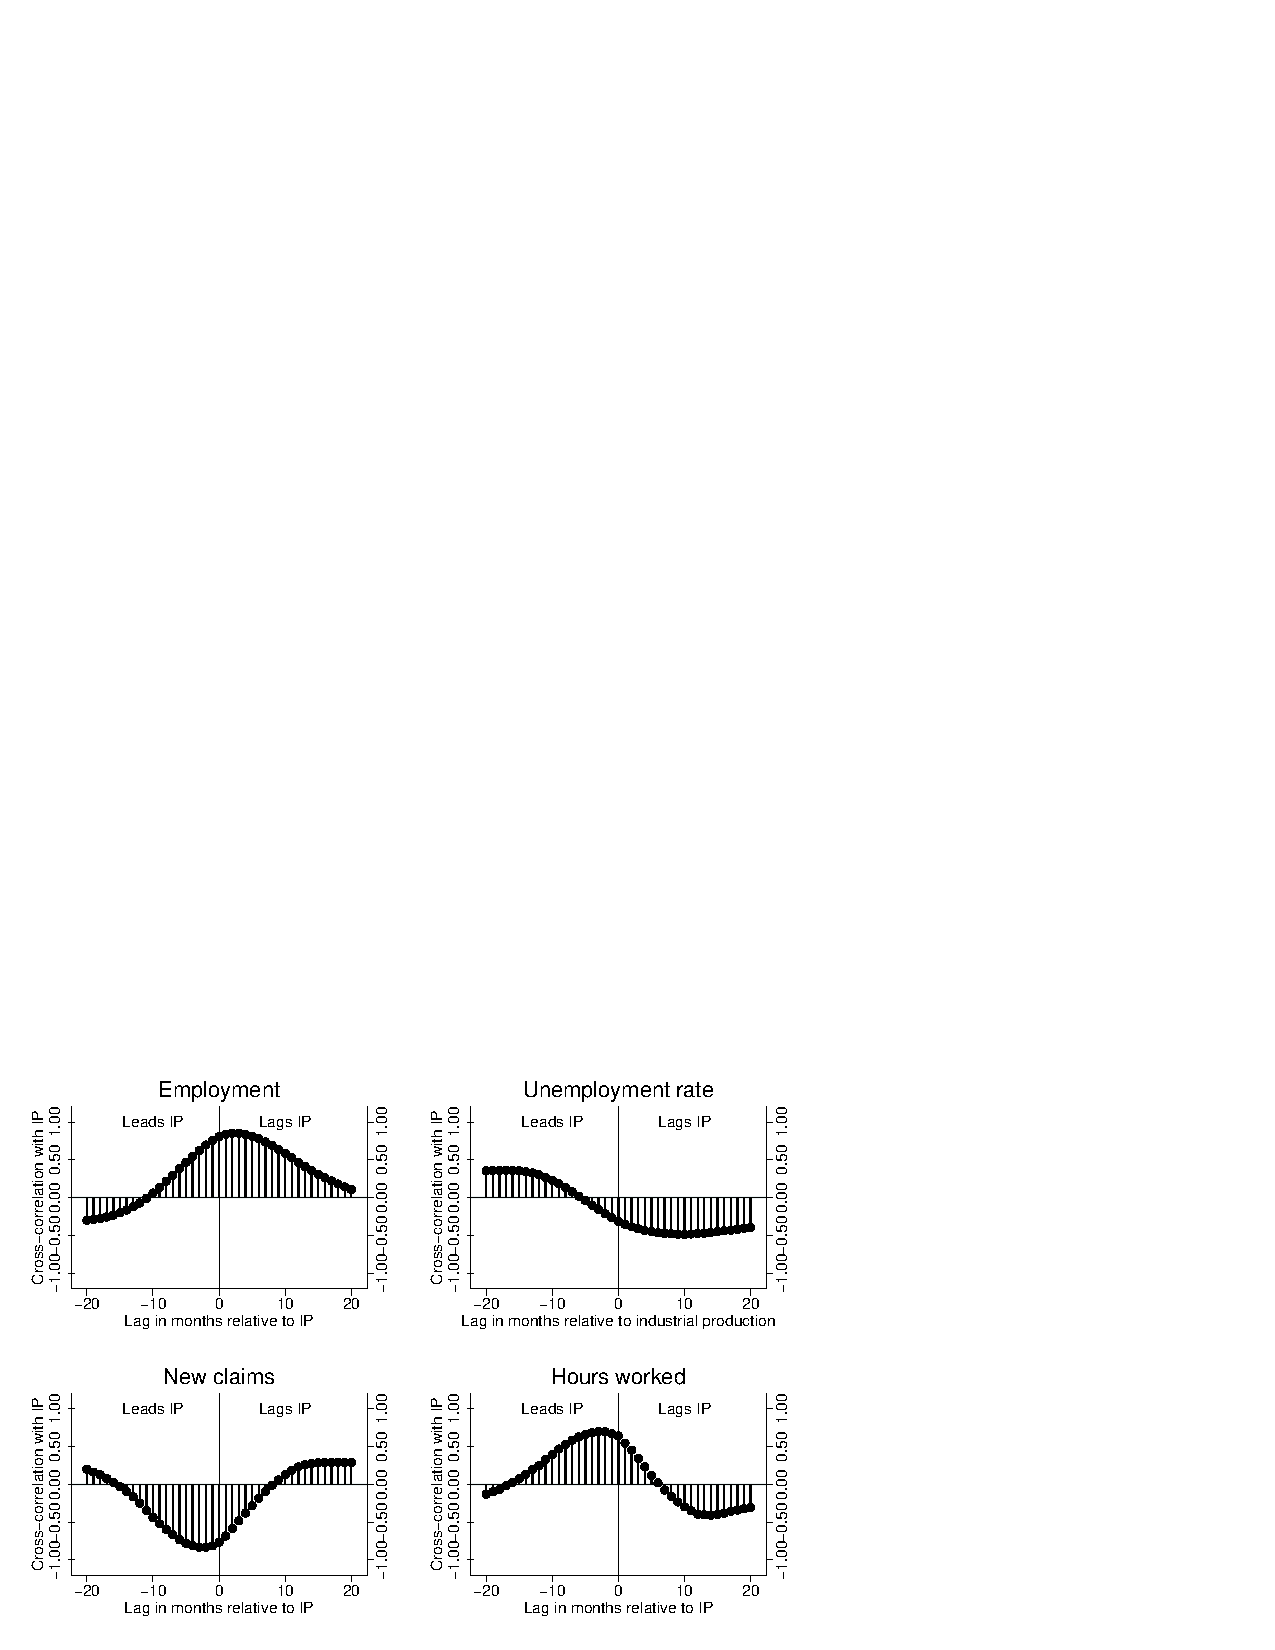
\includegraphics[width=0.9\textwidth]{Figures/xclabor.pdf}
\end{figure}

\begin{figure}
     \caption{Cross-correlation functions:  surveys of economic activity.}
    \label{fig:ccf-survey}%
    \centering
    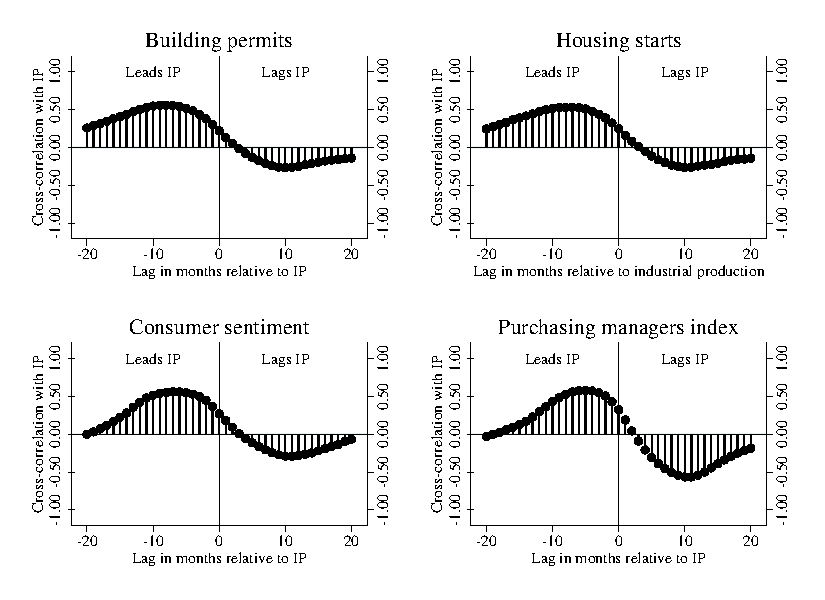
\includegraphics[width=0.8\textwidth]{Figures/xcsurvey.pdf}
\end{figure}

Other sources of useful information are various measures and surveys
of economic activity conducted by the Bureau of the Census and
private organizations.
Cross-correlation functions for four common ones are pictured in
Figure \ref{fig:ccf-survey}.
The first two are \href{http://research.stlouisfed.org/fred2/series/PERMIT}{building permits} and \href{http://research.stlouisfed.org/fred2/series/HOUST}{housing starts},
two indicators of new home construction reported by the Census.
Two ideas lie behind their use:
that construction of new capital is more volatile than other sectors
of the economy
and that decisions to build new homes reflect optimism about the future.
The cross-correlation functions suggest that they work;
while the correlations are
smaller than with (say) employment, the leads are substantial
(ten months or so).
The next two are popular private surveys.
\href{http://research.stlouisfed.org/fred2/series/UMCSENT}{Consumer sentiment}, based on a survey of consumers
collected by the University of Michigan, reflects consumers' optimism about current and future economic conditions.
The \href{http://research.stlouisfed.org/fred2/series/NAPM}{purchasing managers index} is what we call a ``diffusion index.''
It's based on a survey of purchasing managers who report whether
they see economic activity increasing or decreasing.
Each is used as is.
We see in the figure that both are procyclical leading indicators.

We could go on.  There are hundreds of indicators, more all the time.
The most common one we've skipped is the slope of the yield curve:
Flat or downward-sloping yield curves are associated with slower-than-usual
future growth in output. More on this in the Appendix.


\section{The business-cycle scorecard}

Now that we understand how to identify good indicators,
how do we put them to work?
The central question here is how to combine the inputs of multiple indicators.
One way to do that is to summarize them informally, which is what we do here.
Another is to use multivariate regression, which is the next topic.

The business-cycle scorecard is a summary of
what selected indicators tell us about near-term economic conditions.
We'll use the four monthly indicators pictured
in Figures \ref{fig:ip_emp} and \ref{fig:newclaims_hs}.
In the first figure, we see the monthly growth rate
of IP (top panel) and the change in (nonfarm) employment
for the period 1960 to the present.
They show similar patterns, with the major postwar
downturns evident in each.
Evidently, employment is procyclical,  rising in good times
and falling in bad times.
Industrial production is a ``noisier'' series, which is one reason that
many analysts prefer employment as a measure of current economic
conditions. The lines show us the mean value (the solid line)
and plus and minus
one standard deviation (the dashed lines).
The lines are useful benchmarks for telling how strong the
value of an indicator is relative to past experience.

\begin{figure}[h!]
     \caption{Industrial production and employment.}
    \label{fig:ip_emp}%
    \centering
    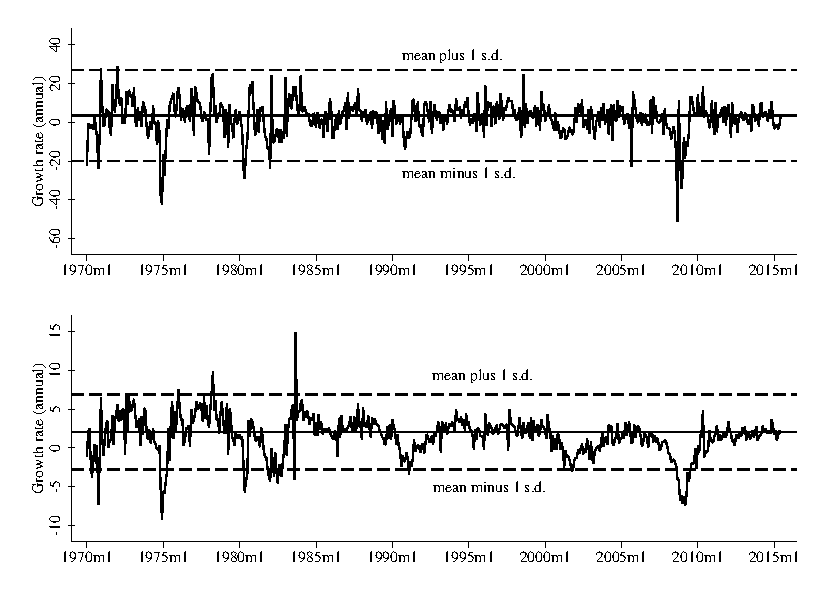
\includegraphics[width=0.9\textwidth]{Figures/scorecard_1.pdf}
    \begin{minipage}{0.85\textwidth}
    {\footnotesize The two panels show, respectively,
    the annual growth rate of industrial production and
    the year-over-year change in the number of people employed.}
    \end{minipage}
\end{figure}

\begin{figure}[h!]
    \caption{New claims and housing starts.}
    \label{fig:newclaims_hs}%
    \centering
    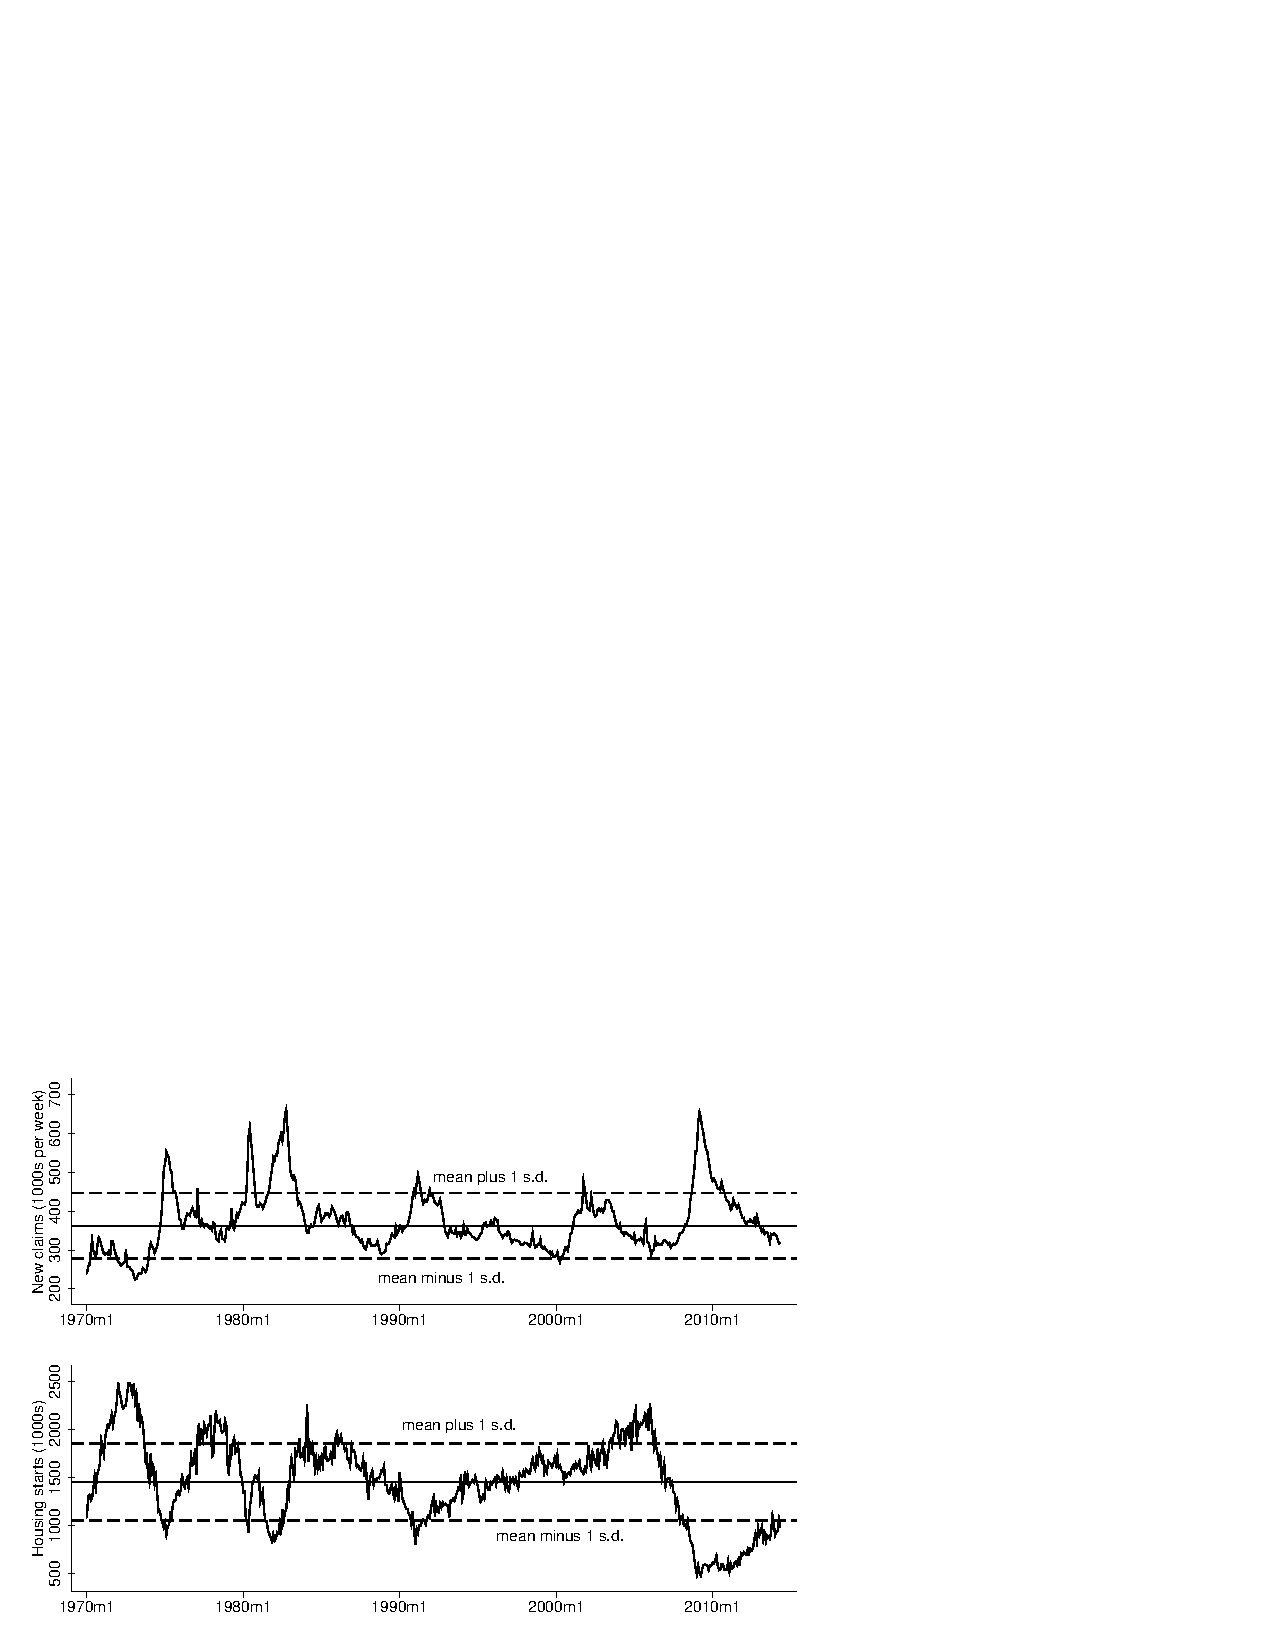
\includegraphics[width=0.9\textwidth]{Figures/scorecard_2.pdf}
    \begin{minipage}{0.85\textwidth}
    {\footnotesize The two panels show, respectively,
    new claims for unemployment insurance
    and housing starts, two popular indicators of economic conditions.}
    \end{minipage}
\end{figure}


In the second figure (Figure \ref{fig:newclaims_hs}),
we see similar data for new claims for unemployment insurance
and housing starts.
New claims are reported weekly; the figure is
based on the four-week moving average.
The second panel is housing starts.
You can see in the figure that housing starts don't always go up
and down with the economy.
In the 2001 recession,
housing starts fell only slightly.
In 2008, we made up for that,
with housing starts falling to their lowest point
since (at least) 1960.
None of that will come as a surprise to you.
These four indicators come from the Federal Reserve (industrial production),
the Bureau of Labor Statistics (employment, new claims),
and the Bureau of the Census (housing starts).
These government agencies are the primary sources of economic indicators
in the US.
There are private indicators also,
but the government indicators are widely used and publicly available.

In the business-cycle scorecard,
we rate each indicator as strong positive if
the current value of the indicator is above the
``mean plus one standard deviation'' line,
weak positive if it's between the mean line and the one above it,
weak negative if it's below the mean line but above
the ``mean minus one standard deviation'' line,
and strong negative if it's below the bottom line.
That's a rough cut, to be sure, but a useful one.
That leads to this summary of economic conditions as of June 2012
based on the four indicators we have seen so far:
\begin{itemize}
\item Industrial production:  Production varied in recent months, but shows a modest growth trend.
Assessment:  weak positive

\item Employment growth:  The most recent number remains soft, amid a disappointing recovery. Assessment:  weak negative.

\item New claims:  They have fallen dramatically
over the last two years, but remain just above the long-run average.
Assessment:  weak positive.
\item Housing starts:  They remain very low by historical standards,
although there has been modest improvement in the recent past.
Assessment:  strong negative.
\end{itemize}


\begin{table}[h!]
\centering
\caption{Business-cycle scorecard in action} %:  US economic conditions in January 2010.}
\begin{tabular}{lcccc}
\toprule
            &  Strong    &  Weak  &  Weak   &  Strong  \\
Indicator   &  Negative  & Negative & Positive & Positive \\
\midrule
Industrial production  &&& x \\
Employment             && x &  \\
New Claims             && x \\
Housing starts         & x &  \\
\midrule
Summary                & 1 & 2 & 1 & 0 \\
\bottomrule
\end{tabular}
\label{tab:scorecard}
\end{table}

These assessments are collected in Table \ref{tab:scorecard}
for a recent date.
Overall, we see three negatives and one positives,
a mixed set of signals that's unusual.
A more extensive analysis would use more indicators,
decide how much weight to give each one,
assess how far into the future they point, and so on.


\section{Regression-based forecasting}

A more formal statistical approach is to include
as many indicators as we like in a multivariate regression.
We estimate the regression by some appropriate method
and use it to forecast the future.
Here are the steps we might follow in constructing a forecast
of (say) industrial production $k$ months in the future.

The first step is to construct the variable we're forecasting.
Let us say that we're interested in the growth rate of industrial
production between now and $k$ months in the future.
You can do what you want, but we compute the (annualized) growth
rate this way:
\[
    \gamma_{t,t+k} \;=\; \ln (\IP_{t+k}/\IP_t) \times (12/k) .
\]
We refer to $k$ (here measured in months) as the {\it forecast
horizon\/}.  The adjustment factor ``$12/k$'' converts the growth
rate to annual units.
For a one-year forecast, then, we would set $k=12$ and compute the
year-on-year growth rate.

The second step is to find some variables you think would be useful
in forecasting.
The previous section might give you some ideas.
There's a half-step that sneaks in about here, too:
what form of the indicator to use.
In most cases, we use growth rates of the indicators, too,
either over one period or a year,
whichever you think works best.
But some variables are used as is.
In Figure \ref{fig:ccf-labor}, for example,
the cross-correlation for the unemployment rate is for the rate, period --- not its growth rate, change, or other transformation.

Third, you put all the ingredients into a statistical package and run a regression.
For example, to forecast IP growth, we would estimate the regression
\[
        \gamma_{t,t+k}  \;=\;  a + b x_t + \mbox{residual},
\]
where $x_t$ is the value of the indicator we have chosen.
We use a sample of data to estimate the parameters $a$ and $b$.
Note well:  The growth rate is between now (date $t$)
and a future date ($t+k$),
but the indicator is observed now (at $t$).
This is central to the exercise:  We use what we know now
to predict the future.
It's not kosher to use future variables to predict the future
because we don't know the future when we make the forecast
(duh!).


Fourth and last:
Once we have estimates of the regression
parameters ($\widehat{a}$ and $\widehat{b}$, say),
we use them and the current value(s)
of the indicator(s) ($x$, say)
to compute the forecast:
\[
        \widehat{\gamma}_{t,t+k}  \;=\;  \widehat{a} + \widehat{b} \; x_t .
\]
The ``hats'' remind us that we are using estimates;
$\widehat{\gamma}_{t,t+k}$ is our forecast of future growth.
There are lots of variants of this approach --- you can add multiple indicators,
lags of the indicators  ($x_{t-1}, x_{t-2}, ...$),
and even past values of the growth rate of industrial
production.
We recommend all of the above.


The result of such an exercise is generally a useful forecast --- useful in the sense that it tells us something about the future.
Something, but not everything!
Over periods of a year or two, forecast accuracy is usually modest.
Even in-sample, the regressions rarely have $R^2$s above 0.25,
which tells us that most of the variation (at least 75 percent) in our forecast variable is unexplained.
Some people see a lesson in this:  It might be more important
to know how to respond when the unexpected occurs
than to have better forecasts.
In practice, both are useful:  knowing something about the future,
and having backup plans to deal with the inevitable forecasting errors. It pays to carry an umbrella when the forecast calls for rain.


\section{Aggregation and prediction markets}

There's another appealing approach to forecasting: Let markets do the work.
Most of the best forecasts aggregate information from multiple
indicators and sources.
Indexes of leading indicators do this one way by combining multiple indicators to produce an index, which is then used
to forecast the future.
Or we could use multiple indicators in regression-based forecasts,
as we suggested above.

Another approach is to aggregate the forecasts themselves --- that is take several forecasts, perhaps based on different indicators, and average them.
The business-cycle scorecard is a simple version of this.
The so-called ``Blue Chip" forecast is an average of forecasts generated by experts, and it performs better than any single forecaster.
Some statistical forecasters do the same sort of thing on their own.
They generate multiple forecasts with methods like our forecasting regression, and then average them to generate a final aggregate forecast. Again,
the aggregate tends to do better than the individual forecasts.

A related idea is to rely on markets, which aggregate information
from the people using them.  \href{http://tippie.uiowa.edu/iem/markets/pres12.html}{Presidential futures markets}, for
example, have predicted the popular vote in the last four
elections more accurately than any of the major polls.
In the economic arena, there are a growing number of markets
in which you can trade futures contracts whose payoffs are tied
to the value of specific economic numbers:
the consumer price index, the fed funds rate, and so on.
These markets are increasingly used as forecasts themselves, with one wrinkle.
The simplest interpretation is that the futures price is a market forecast
of the relevant economic number.
For example, if we are interested in the value of an economic number $y$
to be released in 6 months ($y_{t+6}$, say),
we might use its current futures price ($f_t$, say):
\[
    f_t  \;=\;  \mbox{Market's Current Forecast of } y_{t+6} .
\]
Experience (and possibly some insight) tells us that we may want to make a
correction for the risk of the contract:
\[
    f_t  \;=\;  \mbox{Market's Current Forecast of } y_{t+6}
                + \mbox{Risk Premium} .
\]
There's no limit to the amount of sophistication
we can bring to bear on the last term,
but for now, you can simply note that
we probably want to address it in some way.
Once you do, markets are an extremely useful source of information
about the future.
%An application to the yield curve is included in the Appendix at the end of this chapter.


\section*{Executive summary}

\setlength{\leftmargini}{.5\oldleftmargini}
\begin{enumerate}
\item Fluctuations in economic activity can be (partially)
predicted by a number of indicators.

\item The cross-correlation function is a tool for describing the
timing of the relation between two indicators:
for example, whether one indicator leads another.

\item Markets are useful aggregators of information --- and increasingly popular sources of economic forecasts.
\end{enumerate}
\setlength{\leftmargini}{\oldleftmargini}

\section*{Review questions}

\setlength{\leftmargini}{.5\oldleftmargini}
\begin{enumerate}
\item Terminology. Consider economic indicators in general.
\begin{enumerate}
\item What is a procylical indicator? A countercyclical indicator?
\item Give an example of each.
\item What is a leading indicator?  A lagging indicator?
\item Give an example of each.
\end{enumerate}

Answer.
\begin{enumerate}
\item A procylical indicator moves up and down with GDP.
A countercyclical indicators goes up when GDP moves down.
We typically identify this feature with the sign of the correlation.
\item Most indicators are procyclical:  employment, the S\&P 500, and so on.
The unemployment rate is the classic countercyclical indicator.
\item A leading indicator is correlated with future GDP growth,
a lagging indicator is correlated with past GDP growth.
\item The stock market is a leading indicator,
the unemployment is a lagging indicator.
We typically identify this feature with the cross-correlation function.
\end{enumerate}


\item Housing starts.
We mentioned housing starts as an indicator
of future economic activity.
In what ways do you think it's a good indicator?  A bad one?
(For further information, see the US Census Bureau's
\href{http://www.census.gov/const/www/newresconstindex.html}
{web site}.)

Answer.  Good:  connected to housing, which, as a durable good,
should be cyclically sensitive and volatile; available quickly; it
leads the cycle (as you can see from its ccf). Bad: based on a sample,
which leads to short-term noise; revised periodically;
strong seasonality;
possibly misleading now that we have a glut of housing to work off.

\item Unemployment.  The unemployment rate is widely reported in the press,
but professionals rarely use it.  Why do you think that is?

Answer.
One reason is that the unemployment rate understates the
change in employment in a downturn.
Some people who lose jobs leave the labor force,
so they're not included in the unemployment rate.
Another reason is that the unemployment rate is a lagging
indicator.
It falls slowly, well after the economy turns around.
Employment (the number of people actually working) is
the preferred indicator for both reasons.

%\item The term spread (a long yield minus a short yield)
%is positively correlated with future output growth.  Why do you think that is?
%
%Answer. A steep yield curve means that we expect
%short-term interest rates to rise.  Short-term interest rates may
%rise because the economy is growing quickly (interest rates are
%typically higher in booms) and/or because we expect higher
%inflation (sometimes associated with a booming economy).

\item Terrorism futures.
In 2002, a government agency recommended that we establish a
futures market in terrorist attacks, on the grounds that it would
give us a useful public indicator of their likelihood.  The idea
was widely criticized.  Do you think it was a good idea or a bad
one?  What would you need to do to implement it?

Answer.  Another case of a good idea thrown out because it sounded
bad to politicians.  It's not clear that such attacks are predictable,
but if they are, we'd expect futures markets to do as well as any
other method.  To implement the idea, you'd need to define (and
possibly quantify) a terrorist event.
\end{enumerate}
\setlength{\leftmargini}{\oldleftmargini}

\section*{If you're looking for more}

There are many sources of leading indicators around the world
and lots of guides to them.
Among them:
%
\begin{itemize}

\item The best book we've seen on the subject is
Bernard Baumohl,
\href{http://www.amazon.com/The-Secrets-Economic-Indicators-Opportunities/dp/0132932075/}
{\it The Secrets of Economic Indicators\/}.
If you use economic indicators in your job, you should buy this book.

\item The Bloomberg
\href{http://www.bloomberg.com/markets/ecalendar/index.html}
{Economic Calendar}
gives release dates and short summaries of a wide range of indicators.
Ditto the WSJ, Yahoo, etc.

%\item The Conference Board,
%\href{http://www.conference-board.org/pdf_free/economics/bci/BCI-Handbook.pdf}
%{\it Business Cycle Indicators Handbook\/}.

\item The CME has a nice report,
``Impact of economic indicators on CME group markets,''
on the information content of common indicators for futures prices.
%\href{http://www.cmegroup.com/trading/economic-events/files/Economic-Indicators-WhitePaper.pdf}


%\item Jim Stock and Mark Watson are the two leading academics working on
%economic indicators.  Their 2003 paper in the Richmond Fed's {\it Economic Review\/}
%is an interesting look back at the 2001 recession
%and why many didn't see it coming.
%Here's a
%\href{http://www.richmondfed.org/publications/economic_research/economic_quarterly/pdfs/summer2003/stockwatsonsummer03.pdf}.
%{link}.
%\item The National Bureau of Economic Research
%runs an email alert service
%for major macroeconomic data releases, primarily for the US.
%%See \href{http://nber.org/releases/}{link}.
\end{itemize}
%
To do it right, this topic requires some knowledge of time series statistics.
If you'd like to learn more about forecasting economic and
financial variables specifically,
we recommend ``Forecasting Times Series Data,'' course STAT-GB.2302,
taught in alternate years by Professors Deo and Hurvich, two of our best statisticians.

\section*{Symbols and data used in this chapter}

\begin{table}[H]
\centering
\caption{Symbol table.}
\begin{tabular*}{1.02\textwidth}{l@{\extracolsep{\fill}}l}
\toprule
Symbol & Definition\\
\midrule
$\mathrm{ccf}$             &Cross-correlation function (dynamic correlation of two variables)\\
$\mathrm{ccf}(k)$         &Correlation of ($x_t, y_{t-k}$)\\
$\gamma_{t,t+k}$         &Continuously compounded growth rate, period $t$ to period $t+k$\\
$\hat{x}$                & Estimate of $x$\\
$f_t$                     & Futures price at time $t$\\
$p_m$                     &Price of an m-year zero-coupon bond\\
$y_m$                     &Yield of an m-year zero-coupon bond\\
$f_n$                     &One-period forward interest rate n-periods ahead\\
$f_{n,t}$                 &One-period forward rate arranged at time $t$ for $n$ periods ahead\\
$i_t$                     &One-period interest rate that prevails in period $t$\\
$\mathrm{E}_t(x)$         &Expected value at time $t$ of $x$\\
\bottomrule
\end{tabular*}
\end{table}

\begin{table}[H]
\centering
\caption{Data table.}
\begin{tabular*}{0.7\textwidth}{l@{\extracolsep{\fill}}l}
\toprule
Variable & Source\\
\midrule
Industrial production        &INDPRO\\
Real GDP                    &GDPC1\\
S\&P 500                        &SP500\\
Employment                    &PAYEMS\\
Unemployment rate            &UNRATE\\
New claims                    &IC4WSA\\
Hours worked                &AWHMAN\\
Building permits            &PERMIT\\
Housing starts                &HOUST\\
Consumer sentiment            &UMCSENT\\
Purchasing managers' index    &NAPM\\
10yr Treasury yield            &GS10\\
2yr Treasury yield            &GS2\\
Federal funds rate            &FEDFUNDS\\
\bottomrule
\addlinespace
\end{tabular*}
\begin{minipage}{0.7\textwidth}
\footnotesize{To retrieve the data online, add the identifier from the source column to \url{http://research.stlouisfed.org/fred2/series/}.  For example, to retrieve nonfarm employment, point your browser to \url{http://research.stlouisfed.org/fred2/series/PAYEMS}}
\end{minipage}
\end{table}


\begin{comment}
\newpage
\section*{Appendix:  Reading the yield curve }
\phantomsection
\label{sec:yield_curve}

\subsection*{The yield curve}

We use the yield curve to infer ``the
market's'' forecast of future short-term interest rates.
Roughly speaking, the slope of
the yield curve tells us what the market expects of future
short-term interest rates. But before we explain how this works,
we need to review yields and forward rates.
Most of this should be familiar if you've taken
``Foundations of Finance.''

Yields and forward rates are subspecies of interest rates. {\it
Yields\/} are simply a way of reporting bond prices. If you go
into the bond business, you'll find there are lots of details to
worry about (accrued interest, day count conventions, etc.), but
we'll keep it simple and look at yields on bonds with no coupons --- zero-coupon bonds or ``zeros.''  A one-year zero is a claim to (say) \$100 in
one year.  A two-year zero is a claim to \$100 in two years.  An
$m$-year zero is a claim to \$100 in $m$ years, and so on.  If the
price of an $m$-year bond is $p_m$, its yield $y_m$ is defined by
the present-value formula:
\begin{equation}
        p_m  \;=\; 100/(1+y_m)^m.
        \label{eq:pv}
\end{equation}
This formula is based on annual compounding, which is the most
convenient convention for our purposes; more on this shortly. Note
that if we know prices, we can find yields, and vice versa. The
{\it yield curve\/} for zero-coupon bonds is a graph of yield
$y_m$ versus maturity $m$.


The yield curves you see in the newspaper are usually based on
yields of coupon bonds, and in the case of US treasuries, they use
semi-annual compounding. They capture similar information, but
they're a little harder to make sense of.  Why?  Because the yield
depends not only on maturity, but also on the coupon. Since
the coupons vary over time and across maturities, it's never
exactly clear what we're talking about.  For that reason, most
formal fixed-income analysis starts with prices and yields of
zeros.


\textbf{Example.} Prices of zero-coupon bonds are given in Table \ref{tab:bond prices}. What are the yields?
%
\begin{table}[H]
\centering
\caption{Example bond prices.}
\begin{tabular}{cc}
\toprule
               Maturity        &     Price         \\
\midrule
                1              &      94.24        \\
                2              &      87.70        \\
                3              &      81.22        \\
                4              &      75.16        \\
                5              &      69.66\\
\bottomrule
\end{tabular}
\label{tab:bond prices}
\end{table}
%

Answer.  The yields are 6.11, 6.78, 7.18, 7.40, and 7.50,
respectively, expressed as annual percentages.  The third one
solves the equation $ 81.22 = 100/(1+y_3)^3 $, namely $ 1 + y_3 =
(100/81.22)^{1/3} $.  The others are similar.


Yields are interest rates that apply over a number of periods. For
example, the $m$-year yield at date $t$ applies over the period of
time between $t$ (now) to $t+m$ ($m$ years from now).  One way to
think about the return on the bond is that the holder invests $p$ and
gets a rate of return equal to the yield $y$ for every period
until maturity.  In the two-period case, this leads to
\[
    100 \;=\; p_2 \times (1+y_2) (1+y_2) ,
\]
a variant of our present-value formula, equation (\ref{eq:pv}).
Another way to think about the return is that the rates vary
across periods. In the two-period case, the bond might have
different rates of return in the first and second periods. But
what are these returns?  We know that the return on a one-period bond
is $y_1$, so the first-period return should be $y_1$.  What about
the second period?  We need an interest rate that applies to the
second period alone but that remains consistent with the price of
the bond. That is, a rate $f_1$ that satisfies
\[
    100 \;=\; p_2 \times (1+y_1) (1+f_1) .
\]
Putting these two equations together tells us
\[
    (1+y_2)^2 \;=\; (1+y_1) (1+f_1)
\]
or
\[
    1+f_1 \;=\; p_1/p_2 .
\]
We refer to $f_1$ as the one-period-ahead {\it forward rate\/},
since it applies at date $t$ to the time period between $t+1$ and
$t+2$. It's the rate of return on a {\it forward contract\/} in
which we agree at $t$ to invest a fixed amount at $t+1$ for one
period.
For our purposes, you can think of forward contracts
as identical to the more common futures.
The latter differ (a little) in having a mark-to-market requirement,
which aficionados will take seriously, but the rest of us can safely
ignore.

The same logic applies to bonds with maturities greater than two.
The bond price can be expressed as
\begin{eqnarray*}
        p_m &=& 100/(1+y_m)^m \\
            &=& 100/ [(1+y_1)(1+f_1) \cdots (1+f_{m-1})] .
\end{eqnarray*}
The two relations together imply
\begin{equation}
    1+f_{m-1} \;=\; p_{m-1}/p_{m} ,
    \label{eq:fdef}
\end{equation}
where $f_m$ is the $m$-period-ahead forward rate.  Draw a circle
around this equation since you'll be using it soon.  What we're doing
here is using bonds of two consecutive maturities to ``pick off''
the forward rate that applies over the last period.

Putting all the pieces together, we have three ways to express the
same information:  bond prices, yields, and forward rates. Given
data on a complete set of maturities, we can compute any one of
the three from any other.

\textbf{Example (continued).} For the bond prices and yields
reported earlier, verify that the forward rates are the ones reported in Table \ref{tab:forwards}.
%
\begin{table}[H]
\centering
\caption{Example forward rates.}
\begin{tabular}{cccc}
\toprule
  Maturity ($m$)  &  Price ($p_m$)  &  Yield ($y_m$)  & Forward Rate ($f_{m-1}$) \\
  \midrule
     1      &  94.24  &   6.11 &   6.11    \\
     2      &  87.70  &   6.78 &   7.45         \\
     3      &  81.22  &   7.18 &   7.98     \\
     4      &  75.16  &   7.40 &   8.06       \\
     5      &  69.66  &   7.50 &   7.90\\
     \bottomrule
\end{tabular}
\label{tab:forwards}
\end{table}
Note that the maturities of forward rates are one less than those
of bond prices and yields.  We do this because they naturally
start at zero, for reasons that may be clearer to you shortly. The
0-period-ahead forward rate is simply the current one-period
yield:   $f_0 = y_1$.

Answer.  We compute forward rates from prices.  For $m=5$, the
calculation implied by equation (\ref{eq:fdef}) is
\[
    1 + 0.0790 \;=\; 75.16/69.66.
\]
The others are similar.


\subsection*{Reading the yield curve}

Now that we've done all this work, we can use it to predict future
one-period yields.  Put simply but somewhat imprecisely, we're
going to say that forward rates are the market's expectation of
future one-period yields, plus an adjustment for risk that depends
on maturity but doesn't vary over time.  Once we've done the
adjustment, we can read expected future one-period yields from the
forward rate curve. The idea is referred to as the {\it
expectations hypothesis\/} because it's based on the premise that
forward rates include expectations of future one-period yields --- {\it short rates\/} in conventional terminology.

To be more precise, we need to add a little notation. Since we'll be dealing a lot with the
one-period yield or short rate, let us label it $i$, so that $i_t$ is the yield on a one-period
bond bought at date $t$. We label (one-period) forward rates by $f_{m,t}$, meaning the rate on a
forward contract arranged at date $t$ but applying to the period between dates $t+m$ and $t+m+1$.
The expectations hypothesis states that the forward rate is the market's expectation or forecast
of the future short rate plus a risk premium:
\begin{equation}
    f_{m,t} \;=\; E_t (i_{t+m}) + \mbox{risk premium}_m .
    \label{eq:eh}
\end{equation}
The risk premium is assumed to be constant across time but may
vary by maturity.  The notation $E_t$ is meant to convey the
expectation made at date $t$.  If we know forward rates and risk
premiums, we can compute expected future short rates.


That's what the expectations hypothesis is, but where does it come
from?  Let's think about what an investor would demand of a
forward rate.  An investor with a two-period time horizon has (at
least) two choices.  She could buy and hold a two-period bond at
date $t$, thus getting (according to our second interpretation)
returns of $ i_t $ in the first period and $ f_{1,t} $ in the
second.  Alternatively, she could roll over a one-period bond,
getting (again) $i_t$ in the first period and the short rate $
i_{t+1} $ in the second.  These two possibilities can be pictured this way:
%
\begin{center}
\unitlength=0.6mm
\begin{picture}(100,50)
  \put(50,45){\makebox(0,0){Rollover Strategy}}
  \put(25,32){\makebox(0,0){$i_t$}}
  \put(75,32){\makebox(0,0){$i_{t+1}$}}
  \put(0,25){\line(100,0){100}}
  \put(0,25){\makebox(0,0){$ | $}}
  \put(50,25){\makebox(0,0){$ | $}}
  \put(100,25){\makebox(0,0){$ | $}}
  \put(25,18){\makebox(0,0){$i_t$}}
  \put(75,18){\makebox(0,0){$f_{1,t}$}}
  \put(50,5){\makebox(0,0){Buy and Hold Strategy}}
\end{picture}
\end{center}
%
If $ i_{t+1} $ were known, then we would expect the market to
drive the forward rate $ f_{1,t} $ and the future short rate $
i_{t+1} $ together:  $ f_{1,t} = i_{t+1} $. If the future short
rate were higher, then no one would buy the long bond.  Its price
would fall and the forward rate would rise.  If it were lower,
everyone would buy the long bond and bid up its price. In an
uncertain world, similar logic might lead us to guess that the
forward rate is the market's forecast of the future short rate,
with some adjustment for risk:
\[
    f_{1,t}   =  E_t ( i_{t+1} ) + \mbox{\em risk premium}   .
\]
Similar reasoning for longer maturities leads us to equation
(\ref{eq:eh}).


The only remaining issue is estimating the risk premiums.  There
are as many ways to do this as there are finance professors, but a
relatively simple method is to use the average difference between
the short rate and the $n$-period forward rate as an estimate of
its risk premium; that is, we use
\begin{equation}
    \mbox{risk premium}_m  \;=\; E (f_{m,t}  -  i_{t} )
\end{equation}
and estimate the expectation on the right with the mean. This
should work as long as forecast errors (the difference between the
future short rate and its expectation) are zero, on average, and
the distribution of the short rate doesn't change over time (the
means of the short rate and future short rate are the same).
Table~\ref{tab:meanrates} summarizes mean forward rates for US
treasuries for the period 1970-2000.  Since the short rate is the
first forward rate, we compute risk premiums by subtracting it
from the other forward rates.

\begin{table}[H]
\centering
\caption{Mean forward rates for US Treasuries, 1970-2000.}
\begin{tabular}{ccc}
\toprule
        Maturity   &    Mean Forward Rate   &  Risk Premium \\
\midrule
            1  &  7.51 &  0.00 \\
            2  &  8.10 &  0.59 \\
            3  &  8.39 &  0.88 \\
            4  &  8.57 &  1.06 \\
            5  &  8.67 &  1.16  \\
\bottomrule
\end{tabular}
\label{tab:meanrates}
\end{table}

\textbf{Example (continued).} For the forward rates reported
earlier, what are the implied expected future short rates?

Answer.  The calculations are summarized by:
%
\begin{table}[H]
\centering
\caption{Example expected future short rates.}
\begin{tabular*}{0.9\textwidth}{c@{\extracolsep{\fill}}ccc}
\toprule
  Maturity & Forward Rate & Risk & Future Short Rate \\
    ($m$) &  ($f_{m-1}$) & Premium &  ($i_{t+m-1}$) \\
\midrule
     1      &   6.11       &    0.00      &    6.11 \\
     2      &   7.45       &    0.59      &    6.86  \\
     3      &   7.98       &    0.88      &    7.10  \\
     4      &   8.06       &    1.06      &    7.00  \\
     5      &   7.90       &    1.16      &    6.74\\
\bottomrule
\end{tabular*}
\end{table}

In short, we can read expected future short-term interest rates
from the forward rate curve, which we compute from the yield curve
for zeros.  If you find this interesting, there's a lot more on
related topics in the ``Debt Instruments'' course.
\end{comment}
